%!TEX root = ../Bachelorseminar-RoboticSwarms.tex
As robots become smaller and easier to produce, interest for robotic swarms is created. Many new applications for robotic swarms exist creating a strong growth in the field, indicated by a growing amount of paper written about robotics at for instance the AAMAS (International Conference on Autonomous Agents and Multi-Agent Systems). \cite{Amigoni2014} Many different applications and techniques exist in the field of robotic swarms. This paper aims to deliver a concise review of these applications and techniques. \\

To avoid confusion, some terminology will be defined. Afterwards, in order to emphasize the importance of the connection between the technology and its applications, a top-down approach is used for this survey. Thus, in this paper there will first be decided on the terminology of the research area, after which some applications will be given. In the second part of the paper we will discuss the most used techniques for these applications and the algorithms behind these techniques. At the end a final overview and a discussion will be given.

\subsubsection{Definitions}
%% BELOW WAS FIRST IN DEFINITIONS
This section will provide some definitions so that there will exist no ambiguity for some terms. Firstly, we wish to define what robotic swarms are. A robotic swarm is a collection of robots. In this review, we will only consider something a swarm when the amount of robots is higher than two and the amount can be scalable; so a swarm of only two robots that doesn't interact with a third robot will not count as a swarm.  \\
Furthermore, in this review we will only consider robotic swarms in which each robot is not controlled individually; they should have some form of distributed intelligence. An exception is of course when a swarm of multiple robots is controlled by one control station; this swarm will still have some form of distributed intelligence to function and thus is considered a swarm.  \\

Robotic swarm applications can roughly be characterised by two attributes; they are either \emph{location-based} or \emph{location-free}, or they are either \emph{range-based} and  \emph{range-free}. A location-free approach does not exclude a range-free approach and vice-versa; they are two different ways of approaching an application. The definitions of these attributes may be interpreted ambiguously, which is why we will define it here. The definitions are:

  \begin{itemize}
    \item A robotic swarm is \emph{location-free} if the swarm has no knowledge of the boundaries of te location it is in, whether it is provided at the beginning or is actively searched for during the execution of the algorithm. 
    \item A robotic swarm is \emph{location-based} if the swarm has the knowledge of predefined boundaries of the location it operates in, whether provided at the beginning of the execution of the algorithm or if it is actively searched for. 
    \item A robotic swarm is \emph{range-free} if each robot can detect the presence of other nearby robots or obstactles, but does not store or measure the distance towards the other object.
    \item A robotic swarm is \emph{range-based} if each robot in the swarm keeps track of the exact distance between itself and the other robots in the swarm or obstacles. 
  \end{itemize}

 \subsection{Applications?}
 % DIT STOND EERST ALS INTRODUCTIE BIJ APPLICATIONS
 Robotic swarms can be used for many real-world applications which can be roughly split up in tasks that cover a region, tasks that are to dangerous for human beings, tasks that scale-up or scale-down in time or tasks that require redundancy \cite{csahin2005swarm}. In this chapter, for every technique the scope of the technique is defined and a few examples of practical applications will be named. We should mention that we chose a selection of techniques that we think are mostly used in the applications we have looked at. Some of these techniques partly overlap and/or make use of each other, but it is essential to compare them independently to identify the current problems and already found solutions in swarm robotics.

 \subsection{Techniques?}
 % DIT STOND EERST ALS INTRODUCTIE BIJ TECHNIQUES
 %\begin{figure*}
  \centering
  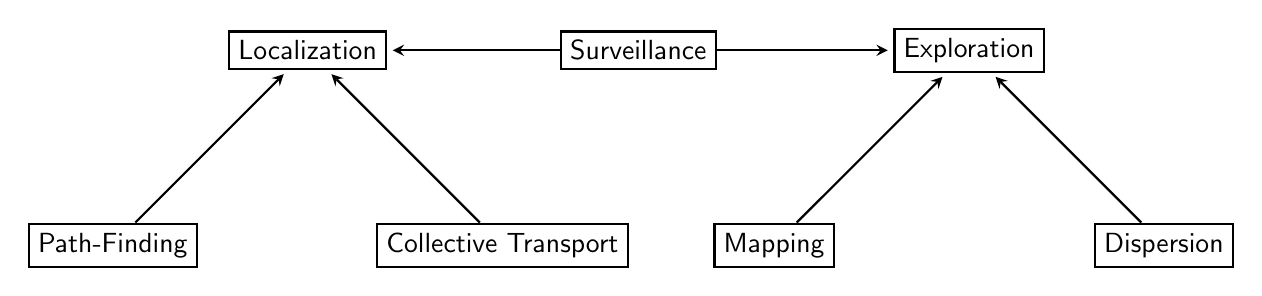
\begin{tikzpicture}[->,>=stealth,shorten >=2pt,auto,node distance=3.5cm,
    thick,main node/.style={fill=white,draw,font=\sffamily}]
    \node[main node] (1) {Localization};
    \node[main node] (2) [below left of=1] {Path-Finding};
    \node[main node] (3) [below right of=1] {Collective Transport};
    \node[main node] (4) [right of=1,node distance=4.2cm] {Surveillance};
    \node[main node] (5) [right of=4,node distance=4.2cm] {Exploration};
    \node[main node] (7) [below left of=5] {Mapping};
    \node[main node] (6) [below right of=5] {Dispersion};

    \path[every node/.style={font=\sffamily\small}]
      (2) edge node [left] {} (1)
      (3) edge [right] node[right] {} (1)
      (4) edge [right] node[above] {} (1)
      (4) edge [right] node[above] {} (5)
      (6) edge [right] node[right] {} (5)
      (7) edge [right] node[left] {} (5);
  \end{tikzpicture}
  \caption{Technique Hierarchy Overview} \label{fig:TechniquesMindMap}
\end{figure*}

After pointing out some applications implementing important techniques used in robotic swarms, we will now provide an in-depth study for these techniques. For every technique, we will make comparisons between different algorithms used by a technique, the problems that are solved and the the problems that are yet to be solved. This chapter thus serves to provide a good overview of ways to implement a technique. 
